\subsection{Křivky}
Křivky dělíme na: \textbf{rovinné}, \textbf{prostorové}, \textbf{interpolační}, \textbf{aproximační}. Jednoduchý příklad křivky je například \textbf{kružnice} nebo \textbf{přímka}. Vyjádření může křivek být v podstatě trojího druhu:
\begin{itemize}
	\item \textbf{Explicitní} -- $y = f(x)$  kde  $x  \in   \mathbb{I}$, např. $y = x^{2} + x + 1$, jedná se o parabolu.
	\item \textbf{Implicitní} -- $F(x, y) = 0$,  $(x+9)^{2} +(y −2)^{2} −4 = 0$, kružnice se středem $[−9, 2]$ a $r=2$.
	\item \textbf{Parametrické}	-- souřadnice bodů parametricky jsou vyjádřeny jako funkce proměnného parametru (například t) definovaného na určitém intervalu. 
	\begin{equation*}
				P(t) = A + \vec{u}t, \quad \textrm{parametr }  t  \in \langle a, b \rangle.
		\end{equation*}
\end{itemize}

\noindent Obecně jsou křivky reprezentovány \textbf{polynomy stupně $ n - 1 $}: $y = a_1x^{n - 1} + a_2x^{n - 2} + \ldots + a_n$,
\begin{itemize}
\item čím vyšší stupeň, tím je křivka více náchylná na ,,rozkmitání'', snažím se proto dávat stupeň co nejmenší,
\item \textbf{derivace} v bodě nám dá \textbf{tečnu} v bodě (lze získat derivací jednotlivých složek přímky), \textbf{první derivace} (směr), \textbf{druhá derivace} (zrychlení směru).
\end{itemize}

\subsubsection{Parametrické křivky}
\begin{itemize}
	\item Mějme interval $I = \langle a, b \rangle \subseteq \mathbb{R}$, pak parametricky vyjádřenou (parametrizovanou) křivku $k$ v $\mathbb{R}^n$ nazýváme \textbf{diferencovatelné zobrazení} $\varphi$  :$I \rightarrow \mathbb{R}^n$.
\begin{figure}[H]
\centering
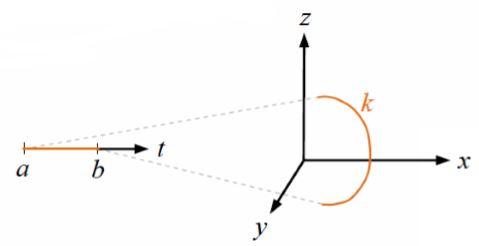
\includegraphics[width=0.4\textwidth]{assets/3_param_curve}
\end{figure}
	\item V trojrozměrném euklidovském prostoru každému číslo $t$ \textbf{odpovídá na křivce příslušný bod} $P(t) = [x(t), y(t), z(t)]$, $t$ je obecně definováno v intervalu $\langle 0, 1 \rangle$. Kde 0 značí \textbf{počátek} a 1 \textbf{konec} křivky.
	\item \textbf{P} je polohový vektor (vektor daný počátkem souřadné soustavy a souřadnicemi příslušného bodu $P$).
\end{itemize}

\subsubsection{Interpolační křivky}
\begin{itemize}
	\item V PG nám pro definování (kreslení) křivky slouží její \textbf{interpolace} (kreslíme jen vybrané body a mezi nimi interpolujeme).
	\item Interpolační křivka k dané množině bodů je taková křivka, která jimi prochází.
	\item Obecně se dá křivka pro $ n $ bodů \textbf{vyjádřit polynomem stupně $ n $}. To znamená, najít řešení soustavy $y = a_1x^{n - 1} + a_2x^{n - 2} + \ldots + a_n$ pro každý bod:
	\begin{equation*}  
			\begin{array}{c}
			  x_{0},x_{1},...,x_{n},  \quad \quad x_{i} \neq x_{j} \quad \textrm{pro }  i \neq j,
			  \end{array}
			\end{equation*}
	\item Hledáme interpolační polynom $P_{n}(x)$ stupně nejvýše $n$, který splňuje \textbf{interpolační podmínky}:
			\begin{equation*}  
			\begin{array}{c}
			  P_{n}(x_{i}) = y_{j} \quad \quad i = 0,1,...,n.
			  \end{array}
			\end{equation*}
	\end{itemize}

\subsubsection{Fergusonova křivka}
\begin{itemize}
	\item Jedná se o jednu z nejpoužívanějších druhů interpolačních křivek, která je \textbf{třetího stupně}.
	\item Generování křivek je \textbf{řízené dvěma krajními body} a \textbf{dvěma vektory} v těchto bodech, jejíž parametrické vyjádření vypadá následovně:
	\begin{equation*}
	P(t) = P_0F_0(t) + P_1F_1(t) + \vec{u}F_2(t) + \vec{v}F_3(t),
	\end{equation*}
kde $P_0$, $P_1$ jsou \textbf{počáteční body}, $\vec{u}$, $\vec{v}$ \textbf{tečné vektory} a $F_0, F_1, F_2, F_3$ nazýváme takzvanými hermitovské polynomy, které jsou dány následujícím předpisem:
\begin{equation*}
\begin{split}
F_0 &= 2t^3 - 3t^2 + 1,\\
F_1 &= -2t^3 + 3t^2,\\
F_2 &= t^3 - 2t^2 + t,\\
F_3 &= t^3 - t^2.\\
\end{split}
\end{equation*}

\item \noindent Výsledný tvar Fergusonovy kubiky, lze ovlivnit \textbf{třemi způsoby:}
\begin{itemize}
	\item \textbf{polohou} řídících bodů $V_0$ a $V_1$,
	\item \textbf{směrem} tečných vektorů $v_0$ a $v_1$,
	\item \textbf{velikostí} tečných vektorů $v_0$ a $v_1$.
\end{itemize}
\item \textbf{Velikost vektorů} $v_0$ a $v_1$ významně \textbf{ovlivňuje} výsledný \textbf{tvar křivky}. Čím délka tečných vektorů je větší, tím více se křivka přimyká k příslušnému tečnému vektoru.
\begin{figure}[H]
\centering
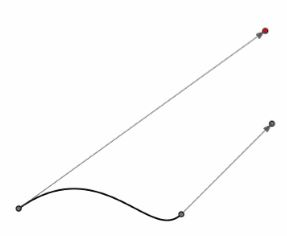
\includegraphics[width=0.3\textwidth]{assets/3_ferg_krivka}
\end{figure}
\begin{figure}[H]
\centering
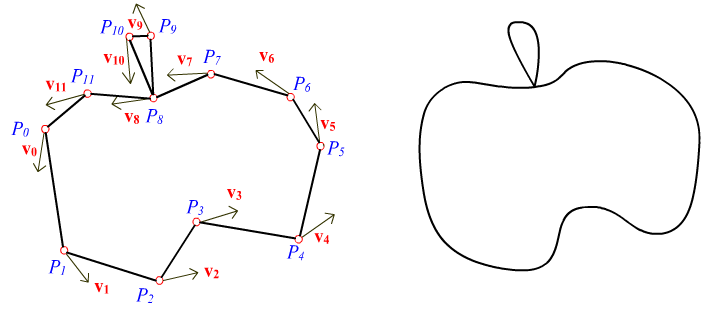
\includegraphics[width=0.6\textwidth]{assets/3_ferg_spline}
\caption{Spline}
\end{figure}
\end{itemize}


\subsubsection{Aproximační přímky}
\begin{itemize}
\item Někdy \textbf{není možné body proložit funkcí} a proto se využívá aproximačních křivek, které \textbf{procházejí v blízkosti bodů}.
\item Je dáno $n$ bodů. Úlohou je nalézt aproximační funkci, která nemusí procházet danými body, ale která co nejlépe vystihuje funkční závislost. 
\end{itemize}

\subsubsection{Metoda nejmenších čtverců}
Před samotným popisem této metody je nutné si připomenout \textbf{explicitně zadanou rovnici přímky}:
\begin{equation}\label{cverce_primka}
f(y) = ax + b.
\end{equation}

Cílem metody nejmenších čtverců je najít takovou rovnici přímky, pro kterou \textbf{součet čtverců odchylek zadané souřadnice $y$ a souřadnice $ax + b$ je co nejmenší}. Tento součet vyjadřuje funkce $f(a,b)$, kde $a$, $b$ jsou koeficienty dané přímky a $n$ je počet zadaných bodů:
\begin{equation}\label{ctverce_suma}
f(a,b) = \sum_{i=0}^{n}(y_i - (a + bx))^2.
\end{equation}

\textbf{Minimum} funkce $f(a,b)$ získáme \textbf{parciální derivací} jejich koeficientů:
\begin{equation}\label{cverce_primka_parc}
\dfrac{\partial f(a,b)}{\partial a}, \quad \quad \dfrac{\partial f(a,b)}{\partial b}.
\end{equation}

Parciální derivací \eqref{cverce_primka_parc} získáme soustavu dvou rovnic, o dvou neznýmých. Výsledné koeficienty této soustavy rovnic dosadíme do explicitní rovnice přímky \eqref{cverce_primka} a získáme hledanou rovnici aproximované přímky.
			
\subsubsection*{Příklad}
Zadání: $A[1,1], \, B[3,2], \, C[2,3].$ Nyní tyto body dosadíme do \eqref{cverce_primka} a získáme vzdálenost mezi zadaným bodem a aproximovanou přímkou.
\begin{equation*}  
1 = a + b,\,\, 2 = 3a + b,\,\, 3 = 2a + b, \,\,
\end{equation*}
Nyní tuto soustavu rovnic můžeme dosadit do vzorce \eqref{ctverce_suma}:
\begin{equation*}  
f(a,b) = (a + b - 1)^2 + (3a + b - 2)^2 + (2a + b - 3)^2.
\end{equation*}
Nyní funkci parciálně derivujeme dle [\ref{cverce_primka_parc}]
\begin{equation*}  
\begin{array}{c}
\frac{\partial c(a,b)}{\partial a} =  2(a + b - 1) + 2(3a + b - 2)3 + 2(2a + b - 3) \quad = 28a + 12b - 26 \\
\frac{\partial c(a,b)}{\partial b} =  2(a + b - 1) + 2(3a + b - 2) + 2(2a + b - 3)  \quad = 12a + 6b - 12
\end{array}
\end{equation*}
Nyní vyřešíme soustavu rovnic a získáme koeficienty aproximované přímky:
\begin{equation*}  
\begin{array}{c}
28a + 12b - 26 = 0 \\
12a + 6b - 12 = 0
2a+1 = 0 \\
a = - \frac{1}{2} \quad \quad b = 3
\end{array}
\end{equation*}
Našli jsme \textbf{aproximaci}:
\begin{equation*}  
f : y = - \frac{1}{2} x + 3.
\end{equation*}

Pokud provedeme \textbf{derivaci} této přímky, dostaneme  $-\frac{1}{2}$. Tato hodnota je taky nazývána jako \textbf{směrnice přímky} a je rovna tangentě mezi přímkou a mezi kladnou poloosou x neboli nám říká, jaký je \textbf{úhel mezi přímkou a poloosou x}. 

\subsection{Tečný a normálový vektor křivky}
\begin{itemize}
	\item Parametrické vyjádření přímky je dáno počátkem v bodě $ A $, vektorem $ \vec{u} $, parametrem $ t $ a předpisem: $P(t) = A + \vec{u}t.$
	\item \textbf{Tečný vektor} v bodě $t=t_0$ je dán jako \textbf{parciální derivace} $P'(t_0) = \frac{dP}{dt}(t_0) = (x'(t_0), y'(t_0), z'(t_0))$
	\item \textbf{Tečna} (přímka, která se v daném bodě křivky dotýká) je dána bodem dotyku a tečným vektorem. $Q(u) = P(t_0) + uP'(t_0)$, kde $u \in \mathbb{R}$
	\item Tečna je limitní polohou sečny (protíná dva body), kdy oba průsečíky splynou v jeden.
\end{itemize}
\begin{itemize}
	\item \textbf{Normálový vektor} je \textbf{kolmý} na tečný vektor. Skalární součin je tedy roven 0. Potřebujeme ho pro \textbf{obecnou rovnici} přímky/roviny. Získáme jej \textbf{prohozením souřadnic směrového vektoru} a u jedné souřadnice změníme znaménko.
\end{itemize}

\subsection{Křivost křivky}
Křivost křivky je jedna ze \textbf{základních vlastností}, které charakterizují křivky. Rozlišujeme dva typy křivostí:
\begin{itemize}
	\item \textbf{první křivost (flexe)} -- obvykle označována pojmem \uv{křivost} a udává velikost odchýlení od křivky $P(t)$ v daném bodě $P(t_0)$. Čím bude mít křivka v daném bodě větší křivost, tím více se v okolí zkoumaného bodu odchyluje od tečny. V \textbf{inflexních bodech} (kde se funkce mění z konvexní na konkávní nebo naopak) je \textbf{křivost nulová}.
		\begin{equation*}
				k_1(t) = \frac{|P'(t) \times P''(t)|}{|P'(t)|^3}
	\end{equation*}
	\item \textbf{druhá křivost (torze)} -- je mírou odchýlení křivky $P(t)$ v daném bodě $P(t_0)$ z její oskulační roviny (viz. oskulační rovina) do prostoru.
	\begin{equation*}
				k_2(t) = \frac{(P'(t) \times P''(t)) \cdot P'''(t)}{|P'(t) \times P''(t)|^2}
	\end{equation*}
\end{itemize}
\subsubsection{Oskulační rovina}
Každá rovina procházející tečnou křivky v bodě $P(t_0)$ se nazývá \textbf{tečná rovina}. Oskulační rovina je \textbf{limitní rovinou} těchto rovin. Pomocí bodu $P(t0)$ a dvou vektorů $P'(t_0)$ a $ P''(t_0)$ zjistíme oskulační rovinu. Jsou--li tyto dva vektory lineárně nezávislé, existuje právě jedna oskulační rovina v daném bodě. V opačném případě je oskulační rovinou každá tečná rovina.


\subsection{Plochy}
\begin{itemize}
	\item \textbf{Rozšířením křivek} se dostaneme k plochám, které mají však s křivkami hodně společného. Zejména některé vznikly rozšířením křivek (Bezier, NURBS).
\end{itemize}
\begin{itemize}
	\item Z parametrického vyjádření je snadné získat jednotlivé body, z implicitního můžeme jednoduše testovat, zda bod patří do plochy nebo ne. 
	\item \textbf{Nejvyužívanější} plochy jsou \textbf{parametrické}. 
	\item Plochy mohou být zadány \textbf{analytickým předpisem}, \textbf{hraničními křivkami}, \textbf{sítí bodů} (NURBS, Bezier) nebo plochy vytvořené \textbf{kinematicky} (rotační plochy, plochy vzniklé skládáním pohybu).
\end{itemize}
Vyjádření ploch analytickým předpisem:
\begin{itemize}
	\item \textbf{explicitní} -- $z = f(x, y)$,
	\item \textbf{implicitní} -- $F(x, y, z) = 0$,
	\item \textbf{parametrické} -- $	P (t) = A + \vec{u}t + \vec{v}t$.
\end{itemize}
Tečné vektory plochy:
\begin{figure}[H]
\centering
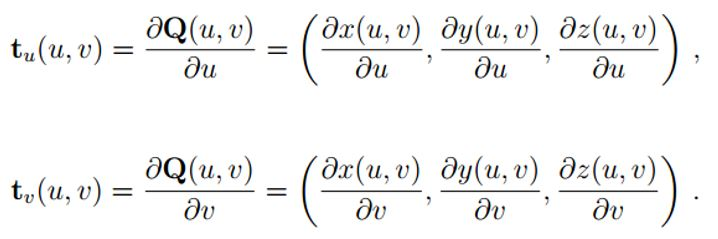
\includegraphics[width=0.6\textwidth]{assets/3_tecne_vektory_plochy}
\end{figure}
Tečná rovina:
\begin{figure}[H]
\centering
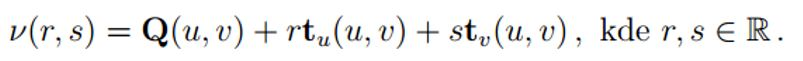
\includegraphics[width=0.7\textwidth]{assets/3_tecna_rovina}
\end{figure}
Normála: Určíme jako \textbf{vektorový součin tečných vektorů}. Jednotkový normálový vektor  $= 
\frac{n}{|n|}$.

\subsubsection{Křivost plochy}
\begin{itemize}
	\item \textbf{Normálová křivost} křivky -- určuje se v \textbf{regulárním bodě plochy pro konkrétní tečnu} a křivku procházející tímto bodem $k_n = k_1(n_k \cdot n) = k_1 \cos{\gamma}$:
	\begin{itemize}
\item 	 $\mathbf{k_1}$ -- první křivost křivky,
\item 	 $\mathbf{n_k}$ -- hlavní normála křivky,
\item 	 $\mathbf{n}$ -- normála plochy,
\item 	 $\mathbf{\gamma}$ -- úhel mezi $\mathbf{n}$ a $\mathbf{n_k}$.
\end{itemize}
	\item \textbf{Gaussova křivost plochy} -- $k_G = k_{n,min} \cdot k_{n,max}$, min. normálová křivost($\mathbf{k_{n,min}}$), a max. normálová křivost($\mathbf{k_{n,max}}$).
	\item \textbf{Střední křivost plochy} -- $k_H = \frac{k_{n,min} \cdot k_{n,max}}{2}$.
	\item \textbf{Absolutní křivost plochy} -- $k_abs = |k_{n,min}| + |k_{n,max}|$.
\end{itemize}
\subsection{Cn a Gn Spojitost}
\begin{itemize}
\item Při navazování oblouků je významným faktorem \textbf{spojitost křivek}. 
\item Výsledná křivka je \textbf{spojitá}, pokud je spojitá \textbf{ve všech svých bodech}, a tedy zejména v navazovacích bodech. 
\item Křivka je \textbf{hladká}, pokud jsou ve všech jejích bodech \textbf{spojité i její první derivace}. Pro vyšší derivace říkáme, že křivka má spojitost druhého, třetího a obecně $n$--tého řádu.
\item Význam spojitosti křivek:
	\begin{itemize}
	\item vizuální stránka napojení dvou křivek,
	\item animace křivky.
	\end{itemize}
\end{itemize}
\subsubsection{Parametrická spojitost $C_n$}
	\begin{itemize}
	\item $\mathbf{c_0}$ -- koncový bod prvního segmentu je počátečním bodem segmentu druhého,	
	\item $\mathbf{c_1}$ -- rovnost tečných vektorů v daném uzlu, 		
	\item $\mathbf{c_2}$ -- rovnost prvních derivací tečných vektorů v daném uzlu.
	\end{itemize}
Čím vyšší spojitost je požadována, tím delší ,,dobu'' (ve smyslu parametru $\mathbf{t}$) se oba segmenty k sobě \textbf{přimykají}. Ze spojitosti $\mathbf{c_0}$ plyne, že bod se pohybuje po spojité dráze, ale v uzlu může měnit skokem směr pohybu, rychlost i zrychlení. Směr pohybu a velikost rychlosti se nemůže měnit skokem při spojitosti $\mathbf{c_1}$ a zrychlení zůstává nezměněné při spojitosti $\mathbf{c_2}$.

\subsubsection{Geometrická spojitost $G_n$}
	\begin{itemize}
		\item $\mathbf{g_0}$ -- koncový bod prvního segmentu je počátečním bodem segmentu druhého,
		\item $\mathbf{g_1}$ -- tečné vektory jsou lineárně závislé.
	\end{itemize}
Opticky zaručuje $\mathbf{g_1}$ spojitost ,,skoro stejno'' hladkost jako $\mathbf{c_1}$. Z hlediska použití bývá jednodušší zaručit spojitost $\mathbf{g_1}$ nežli $\mathbf{c_1}$.

\subsection{Bézier}
Jedná se o nejčastěji používaný typ interpolační křivky zejména v 2D i 3D počítačové grafice. Oproti Fergusonově křivce jsou Beziérovy \textbf{křivky zadány pouze řídícími body}. Tyto křivky vždy prochází počátečním a koncovým bodem a zároveň nikdy neopustí svůj \textbf{konvexní obal}, který je dán řídícími body. Beziérova křivka je dána předpisem:
\begin{equation*}\label{rovnice_bezier}
X(t) = \sum_{i=0}^{n}P_iB_i^n(t),
\end{equation*}
kde $B_i^n$ jsou Bernsteinovy polynomy, které jsou definovány:
\begin{equation*}
B_i^n(t) = \binom{n}{i}(1 - t)^{(n - i)}t^i.
\end{equation*}
\begin{itemize}
\item \textbf{Lineární} Bézierová křivka je přímka z bodu $P_{0}$ do bodu $P_{1}$.
\item \textbf{Kvadratická} Bézierová křivka je definována \textbf{třemi} řídícími body.
\item \textbf{Kubická} Bézierová křivka je definována \textbf{čtyřmi} řídícími body.
\end{itemize}

\subsubsection{Beziérova kubika}
Kubické Bézierovy křivky mají velký význam pro praxi, protože jsou skládány z menších dílů, kde můžeme jednoduše definovat spojitost v řídících (koncových) bodech jednotlivých segmentů. Další výhodou je omezený vliv změny polohy jednoho bodu na tvar celé křivky. Bernsteinovy polynomy pro Beziérovu kubiku vypadají následovně:
\begin{equation*} \label{rovnice_bezier_kubika}
\begin{split}
B_0^3(t) &= -t^3 + 3t^2 - 3t + 1,\\
B_1^3(t) &= 3t^3 - 6t^2 + 3t,\\
B_2^3(t) &= -3t^3 + 3t^2,\\
B_3^3(t) &= t^3.\\
\end{split}
\end{equation*}

\subsubsection{Konstrukce Bézierovy křivky}
\begin{figure}[H]
\centering
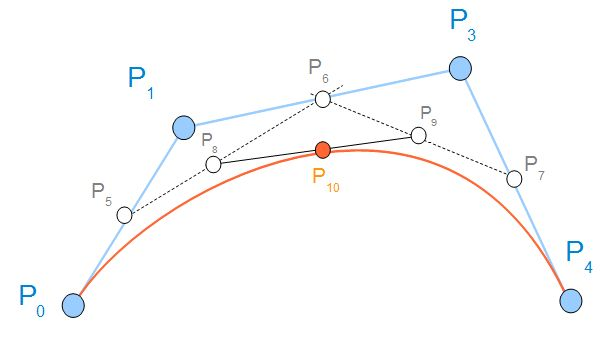
\includegraphics[width=0.5\textwidth]{assets/2_bezier_ex}
\end{figure}
Pro geometrickou konstrukci Beziérovy křivky zvolíme poměr $ t $, v kterém dělíme lomenou řídící čáru, jak je vidět na obrázku nahoře, kde je $t=0,5$. 

Takto jsme vykreslili první bod křivky $\mathbf{P_10}$. Konstrukcí bodu $\mathbf{P_10}$ jsme získali nové řídící body, které použijeme pro získání dalších bodů křivky. Další dva body křivky tedy získáme stejným způsobem za použití řídících bodů {$\mathbf{P_0}$, $\mathbf{P_5}$, $\mathbf{P_8}$, $\mathbf{P_10}$} a {$\mathbf{P_10}$, $\mathbf{P_9}$, $\mathbf{P_7}$, $\mathbf{P_4}$}. Tímto rekurzivním způsobem postupně vykreslíme celou křivku.

Výhoda této konstrukce je, že můžeme ovlivnit hustotu vykreslování dle potřeby. Například v oblasti velkého zakřivení.

\subsubsection{Převod Fergusonovy kubiky na Beziérovu kubiku}
Fergusonovu křivku lze převést na Beziérovu křivku, pokud se budeme při výpočtu držet následujícího pravidla:
\begin{equation*}\label{prevodfergusbezier}
\begin{split}
P_0 &= V_0,\\
P_1 &= V_0 + \frac{1}{3}\vec{u},\\
P_2 &= V_1 - \frac{1}{3}\vec{v},\\
P_3 &= V_1.\\
\end{split}
\end{equation*}

\subsection{Coons}
\begin{itemize}
	\item Coonsnová kubická B-spline křivka vznikne pospojováním Connsnových kubik, tak aby byla zajištěna \textbf{spojitost druhého řádu}.
	\item Coonsnová kubika je parametrická křivka dána čtyřmi body $P_0, P_1, P_2, P_3$ a tímto vztahem:
		\begin{equation*} 
			P(t) = \frac{1}{6} (P_0C_0(t) + P_1C_1(t) + P_2C_2(t) + P_3C_3(t))
		\end{equation*}
		kde bázové funkce jsou:
		\begin{equation*} 
		\begin{split}
			C_0(t) &= -t^3 + 3t^2 - 3t + 1, \\
			C_1(t) &= 3t^3 + 6t^2 + 4, \\
			C_2(t) &= -3t^3 + 3t^2 + 3t + 1, \\
			C_3(t) &= t^3
		\end{split}		
		\end{equation*}
\end{itemize}
\begin{figure}[H]
\centering
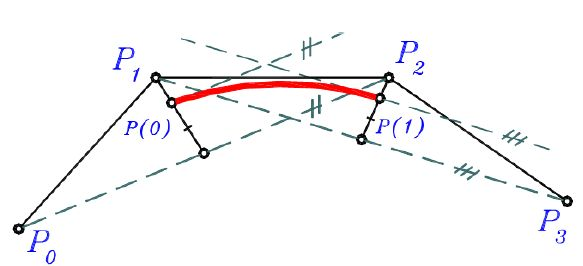
\includegraphics[width=0.7\textwidth]{assets/2_coons-b-spline}
\end{figure}
\subsection{NURBS (Non-uniform rational b-spline)}
\begin{itemize}
	\item Obyčejným beziérem nejde udělat dokonalý kruh, proto se přidávají \textbf{váhy} $w$, kterými se přenásobují jednotlivé Bernsteinovy polynomy. Tento způsob reprezentuje vlastnost \textbf{racionality}.
	\item \textbf{Neuniformnost} znamená, že parametry $t$ můžou nabývat různých hodnot i mimo interval $\langle0,1\rangle$ a pro každou část můžou být jinak \uv{rychlé}.
			\begin{equation*} 
		\begin{array}{c}
			C(t) = \frac{\sum\limits_{i=0}^m w_i P_n N_i^n (t) }{\sum\limits_{i=0}^m w_i N_i^n (t)}, \quad \textrm{kde: } t \in \langle0t_n, t_{m+1}\rangle
		\end{array}		
		\end{equation*}
	\item Bázová funkce $N_i^n$ je definována rekurentně: nechť $t = (t_0, t_1 \ldots t_i)$ je \textbf{uzlový vektor}, b-spline funkce stupně $n$ je definována jako:
		\begin{figure}[H]
		\centering
		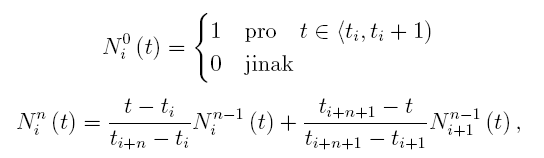
\includegraphics[width=0.7\textwidth]{assets/3_nurbs}
		\end{figure}
	%našel jsem toto, ale jak jsem viděl ty vzorce, meh, nechtělo se mi to ani dělat :D
	% https://www.root.cz/clanky/krivky-nurbs-1/
\end{itemize}